\section{Background}

While our insight and approach is general, in order to demonstrate its
practicality we prototype it in the context of Clover~\cite{clover}, a
disaggregated key/value store.  Hence, we begin with a brief overview
of the relevant aspects of Clover's design for the uninitiated.

\subsection{Append-only updates}

\begin{figure}
    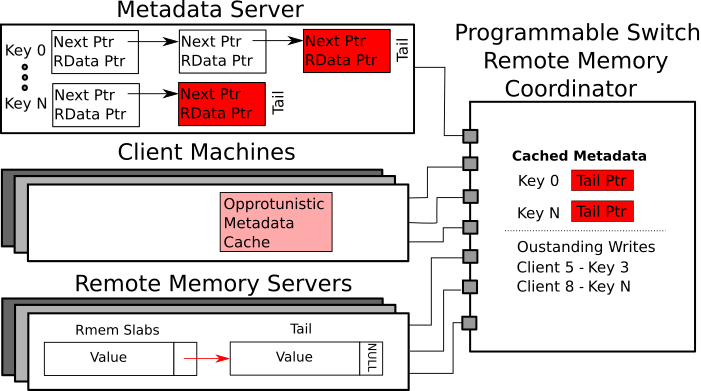
\includegraphics[width=0.45\textwidth]{fig/overview_2.png}
%%
    \caption{ System overview, Metadata, client, and Remote Memory
    servers are Clover components. Our remote memory coordinator is
    located on a centralized TOR interconecting the clover components.
    }
%%
    \label{fig:overview} 
\end{figure}

Clover maximizes read performance by separating key/value metadata
from the datapath, which is implemented as a linked list of value
updates that the authors term a \emph{chain} that supports an atomic
append-to-tail operation illustrated in Figure~\ref{fig:overview}.
Each value update contains a pointer to the next update in the version
chain, and metadata servers keep pointers to the current tail of the
chain for each key allowing clients to issue lock-free RDMA reads
directly to passive remote memory servers using the address they
believe to be the current end of the chain.  Clients can independently
confirm their reads are fresh by ensuring the value returned has a
``null'' next-update pointer.

Write (i.e., append-to-tail) operations, on the other hand, require
multiple steps.  First a writer issues a lock-free RDMA write to store
the new value update in an uncontended portion of remote
memory. After the RDMA operation completes a second operation
optimistically attempts to atomically add the new update to the end of
the chain.  Specifically, the writer issues an RDMA compare-and-swap
(c\&s) operation to the old tail to replace its (presumably still
``null'') next-update pointer with the address of the new value.  If
successful the client lazily updates the metadata sever with the
new end-of-chain address.
%(as any concurrent writes to the
%same location will fail the comparison).

%% This operation ensures that the next
%% write to the data structure writes to the tail of the linked list.
%% This operation requires two steps.

The authors show their opportunistic approach obtains extremely high
throughput with read-heavy workloads as updates are rare and clients
enjoy unfettered access to remote memory. In contrast they find that
placing a metadata coordinator on the datapath becomes a bottleneck at
only a fraction of their achievable throughput.  In the presence of
writes, however, Clover's throughput decreases due to contention.

\subsection{Conflict handling}

If multiple clients attempt to update the value concurrently, each
will succeed in writing their new value to remote memory but then
issue conflicting RDMA c\&s operations to the end of the chain.  The
race is resolved at the remote memory location of the previous update
in the chain: only the first c\&s operation will succeed; all
subsequent operations will fail because rather than finding a value
with a ``null'' next-update pointer, they find the now (at best)
penultimate value in the chain which points to the update issued by
the client that won the race.
%When
%concurrent writes update the same key a race occurs to write at the
%end of the chain. Write operations require two separate RDMA
%transactions that must each complete to ensure atomicity.
During this
two-RTT operation any concurrent write to the same key will cause a
conflict.

%% The process which lost the race now needs to engage in \textit{Pointer
%% chasing} to find the new tail. It must iterative issue reads of the
%% linked list, step by step until it finds the location of the new tail.


If a client's write---or read---fails because it did not succeed in
accessing the current end of the chain they concurrently request the
new address from the metadata server and traverse the chain themselves
through remote memory to find the current end in a processes known as
\emph{chain walking}.  (It is insufficient to just consult the
metadata server because they are updated lazily.)  Failed writers must
then issue a new c\&s operation at the updated end of the chain to append
their pending update.  Of course, the reissued c\&s is subject to the
same race condition as many writers may be executing
concurrently. This pointer-chasing reconciliation algorithm must be
run independently each time a conflict occurs.
%The slower writers will fail the guard, and must retry
%their c\&s operation after walking the chain through remote memory or
%by getting an update from the metadata server.
While concurrent read operations will not prevent a write from
succeeding, a reader that loses the race with a c\&s operation will
need to issue another RDMA read to the new address to obtain the
updated value.  On write-heavy workloads these race conditions happen
frequently
%as illustrated in Figure~\ref{fig:conflicts},
%, which leads to a sharp decrease in throughput.  For highly
%contested structures, the number of retries can grow quickly,
leading to large and unpredictable tail latencies~\cite{clover}.




%\begin{figure}
%    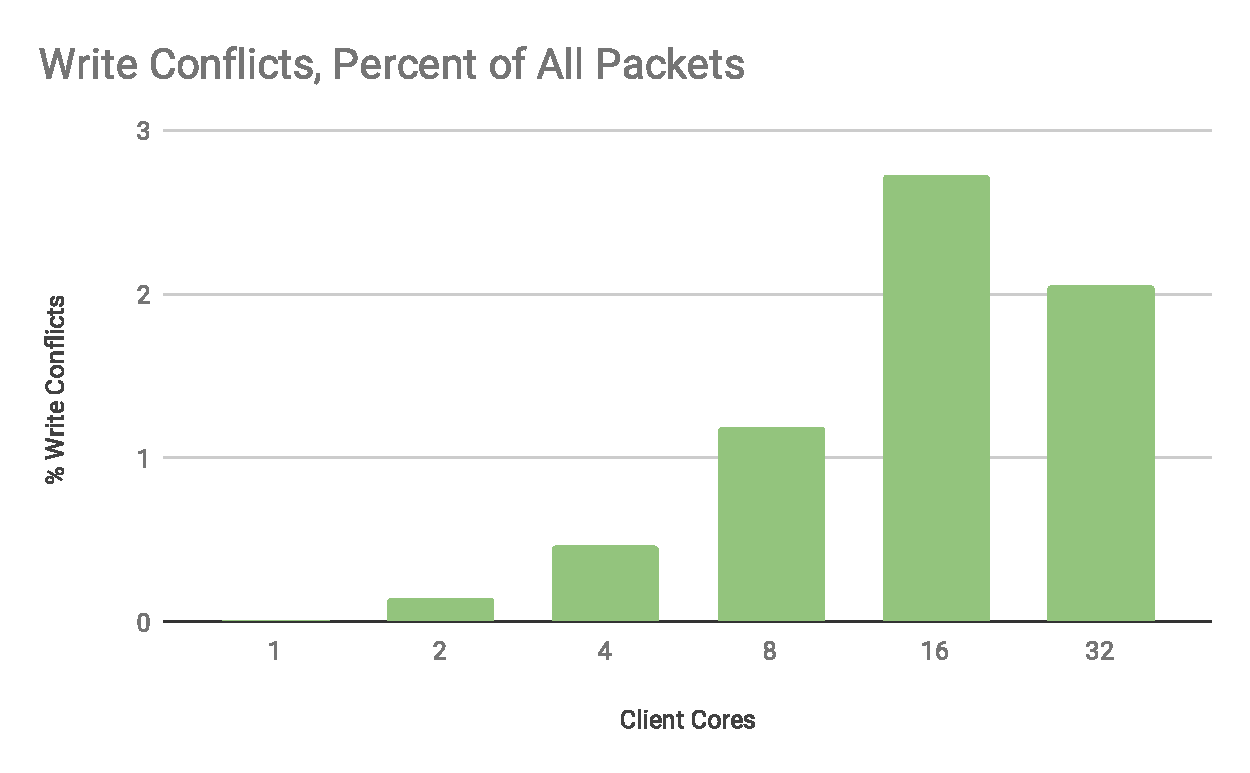
\includegraphics[width=0.45\textwidth]{fig/write_conflicts.pdf}
%    \caption{Clover write conflicts grow with the number of clients
%    (50\% write Zipf 0.99 distribution)\todo{redo with 64 cores and
%    writes only}}
%    \label{fig:conflicts}
%    \vskip -0.5em
%\end{figure}



%% The high level pitch about remote memory.
%Far memory projects typically have a remote CPU which is used to
%coordinate access to remote resources (cite all object systems). In a
%disaggregated system there is no remote CPU, therefore the coordination
%of reads and writes to remote locations must be done locally. For
%performance local caches of remote resources can be used to organize
%access to remote resources. For data structures which require
%consistency this creates a problem as stale caches can lead to data
%structure corruption.

